\chapter{相对论动力学}

上一章中，我们已经看到：长度会收缩，时钟会变慢，同时性不再绝对。到这里，牛顿力学中最根本的两个量——动量与能量——也必须被重新审视。经典力学中，$\vb{p}=m\vb{v}$ 与 $E=\tfrac12 mv^2$ 在低速下极其成功；但当速度接近光速时，它们不再能与洛伦兹变换以及守恒律相容。

本章的任务，是把牛顿时代熟悉的“力、动量、能量”提升到四维时空的框架中，建立狭义相对论的动力学。这样做的结果并不是把经典力学全部推翻，而是把它放进一个更大、更统一的结构里：低速时回到牛顿，高速时显出爱因斯坦。

\section{相对论动量}

经典动量定义为
\[
\vb{p}_{\text{cl}}=m\vb{v}.
\]
在日常速度范围内，它与实验完美吻合；但一旦粒子速度逼近光速，这个定义就会遇到两个困难：
\begin{itemize}
  \item 它无法保证不同惯性系对碰撞过程给出一致的守恒结论；
  \item 它暗示粒子只要持续受力，就可以被加速到超过光速，这与相对论速度叠加公式矛盾。
\end{itemize}

问题的根源在于：时间与空间已经耦合成时空，因此动量也不能再只是一个孤立的三维量。我们需要寻找一个在洛伦兹变换下具有良好性质的定义。

\begin{definition}[相对论动量]
质量为 $m$、速度为 $\vb{v}$ 的粒子的\emph{相对论动量}定义为
\[
\vb{p}=\gamma m\vb{v},
\qquad
\gamma\coloneqq \frac{1}{\sqrt{1-v^2/c^2}}.
\]
其中 $m$ 是粒子的静质量，$c$ 是真空中的光速。
\end{definition}

当 $v\ll c$ 时，
\[
\gamma = 1 + \frac12\frac{v^2}{c^2}+\cdots \approx 1,
\]
于是
\[
\vb{p}\approx m\vb{v},
\]
这说明相对论动量自然退化为经典动量。真正的差别出现在 $v$ 不再远小于 $c$ 的时候：随着 $v\to c$，$\gamma\to \infty$，于是动量会迅速增大，而速度却始终不能超过 $c$。

\begin{remark}
早期文献有时把 $\gamma m$ 称为“相对论质量”。现代物理更倾向于保留不变的静质量 $m$，把速度效应全部放入 $\gamma$ 中。这样概念更清楚，也更适合四矢量表述。
\end{remark}

为什么 $m\vb{v}$ 不够用？可以从守恒律的角度理解。设想两个相同粒子在某参考系中对心碰撞，碰撞前后总动量都为零。换到另一个相对运动的惯性系后，两粒子的速度需要用洛伦兹速度变换来计算；这时若仍使用经典公式 $m\vb{v}$，则碰撞前后的总动量一般不再严格相等。只有使用 $\gamma m\vb{v}$，守恒律才能在所有惯性系中保持一致。

从微分形式上看，相对论中仍保留牛顿第二定律的结构
\[
\vb{F}=\dv{\vb{p}}{t},
\]
但这里的 $\vb{p}$ 必须理解为相对论动量。于是加速度与力不再简单成正比：当粒子越来越快时，同样大小的力产生的速度增量会越来越小。

\begin{example}[高速电子的动量]
一电子以 $v=0.80c$ 运动。求它的相对论动量，并与经典动量比较。

由
\[
\gamma = \frac{1}{\sqrt{1-0.80^2}}=\frac{1}{0.60}=\frac53,
\]
得
\[
 p=\gamma mv = \frac53 m(0.80c)=1.33\,mc.
\]
若用经典公式，则
\[
 p_{\text{cl}}=0.80\,mc.
\]
两者之比为
\[
\frac{p}{p_{\text{cl}}}=\gamma=\frac53.
\]
可见在 $0.80c$ 时，经典动量已经低估了约 $40\%$。
\end{example}

作为一个数量级估算，若一质子从 $0.90c$ 提高到 $0.99c$，则
\[
\gamma(0.90c)\approx 2.29,
\qquad
\gamma(0.99c)\approx 7.09,
\]
从而
\[
 p(0.90c)\approx 2.06\,mc,
 \qquad
 p(0.99c)\approx 7.02\,mc.
\]
虽然速度看起来只增加了不到 $10\%$，动量却增加了三倍多。这正是现代加速器需要巨大能量输入的原因：粒子越接近光速，继续提升速度就越困难。

\begin{figure}[htbp]
\centering
\begin{tikzpicture}
\begin{axis}[
  width=0.75\textwidth, height=0.5\textwidth,
  xlabel={速度比 $\beta=v/c$}, ylabel={动量比 $p/(mc)$},
  xmin=0, xmax=0.98, ymin=0, ymax=5.2,
  axis lines=middle,
  grid=major, grid style={gray!30},
  thick,
  legend style={at={(0.98,0.02)}, anchor=south east, draw=none, fill=none}
]
\addplot[blue, domain=0:0.98, samples=200] {x/sqrt(1-x^2)};
\addlegendentry{相对论动量}
\addplot[red, dashed, domain=0:0.98, samples=200] {x};
\addlegendentry{经典动量}
\end{axis}
\end{tikzpicture}
\caption{相对论动量在速度逼近光速时显著偏离经典结果}
\end{figure}

\section{相对论能量}

经典动能定义为 $K=\tfrac12 mv^2$。它在低速下正确，但在高速下也必须修正。修正的方法可以从功的定义出发：外力对粒子所做的功等于粒子能量的变化。

沿粒子轨迹有
\[
\dd E = \vb{F}\cdot \dd \vb{x}.
\]
又因为 $\vb{F}=\dv*{\vb{p}}{t}$，所以
\[
\dd E = \vb{v}\cdot \dd \vb{p}.
\]
代入
\[
\vb{p}=\gamma m\vb{v},
\]
经过计算可得
\[
\dd E = mc^2\,\dd \gamma.
\]
积分后得到
\[
E=\gamma mc^2 + \text{常数}.
\]
若规定粒子在静止时仍然具有能量 $E_0$，则当 $v=0$、$\gamma=1$ 时，
\[
E_0 = mc^2.
\]
因此总能量写成
\[
E=\gamma mc^2,
\]
而动能为
\[
K=E-E_0=(\gamma-1)mc^2.
\]

\begin{definition}[总能量与静能]
粒子的\emph{总能量}定义为
\[
E=\gamma mc^2,
\]
粒子静止时的能量称为\emph{静能}：
\[
E_0=mc^2.
\]
两者之差
\[
K=(\gamma-1)mc^2
\]
称为粒子的相对论动能。
\end{definition}

把 $\gamma$ 在低速下展开：
\[
\gamma = 1 + \frac12\frac{v^2}{c^2}+\frac{3}{8}\frac{v^4}{c^4}+\cdots,
\]
便得
\[
E = mc^2 + \frac12 mv^2 + \frac38 m\frac{v^4}{c^2}+\cdots.
\]
这告诉我们：经典动能并没有错，它只是总能量减去静能之后的最低阶近似。

\begin{law}[相对论能量表达式]
对静质量为 $m$、速度为 $v$ 的粒子，
\[
E=\gamma mc^2,
\qquad
K=(\gamma-1)mc^2,
\qquad
E_0=mc^2.
\]
当 $v\ll c$ 时，$K\approx \tfrac12 mv^2$。
\end{law}

\begin{figure}[htbp]
\centering
\begin{tikzpicture}
\begin{axis}[
  width=0.75\textwidth, height=0.5\textwidth,
  xlabel={速度比 $\beta=v/c$}, ylabel={能量比 $K/(mc^2)$},
  xmin=0, xmax=0.98, ymin=0, ymax=4.2,
  axis lines=middle,
  grid=major, grid style={gray!30},
  thick,
  legend style={at={(0.98,0.02)}, anchor=south east, draw=none, fill=none}
]
\addplot[blue, domain=0:0.98, samples=200] {1/sqrt(1-x^2)-1};
\addlegendentry{相对论动能}
\addplot[red, dashed, domain=0:0.98, samples=200] {0.5*x^2};
\addlegendentry{经典动能}
\end{axis}
\end{tikzpicture}
\caption{相对论动能与经典动能的比较}
\end{figure}

\begin{remark}
静能并不是“额外附送”的一项，而是物体作为一个存在的物理实体所固有的能量储备。化学能、核能、弹性能，乃至热能的变化，本质上都伴随着系统总质量的极微小变化。
\end{remark}

\begin{example}[静能的数量级]
设一小球质量为 $1\,\mathrm{g}=10^{-3}\,\mathrm{kg}$。它的静能为
\[
E_0 = mc^2 = 10^{-3}\times (3.0\times 10^8)^2\,\mathrm{J}
=9.0\times 10^{13}\,\mathrm{J}.
\]
这是一个极其惊人的数字，约等于一座中型城市长时间用电所需能量的量级。日常生活中我们感受不到它，是因为通常只有极小一部分静能能够通过物理过程释放出来。
\end{example}

\section{质能等价}

公式
\[
E_0=mc^2
\]
常被视为爱因斯坦最著名的结论。它告诉我们：质量不是与能量并列、彼此独立的“另一种东西”；质量本身就是能量的一种形式。更准确地说，质量衡量的是系统在自身静止系中的能量含量。

我们可以从总能量公式直接得到质能等价。对任意粒子，
\[
E=\gamma mc^2.
\]
当粒子静止时 $v=0$，于是 $\gamma=1$，故
\[
E_0=mc^2.
\]
这就是质能等价最简洁的推导。

如果系统向外辐射能量 $\Delta E$，而系统整体仍保持静止，那么其静质量会减少
\[
\Delta m = \frac{\Delta E}{c^2}.
\]
反过来，如果系统吸收能量，它的总质量也会增加。这种变化通常极小，但在核反应与粒子反应中却能被清晰观测到。

\begin{theorem}[质能等价的系统表述]
任一孤立系统在其质心静止系中的总能量 $E_{\mathrm{rest}}$ 与系统的不变质量 $M$ 满足
\[
E_{\mathrm{rest}} = Mc^2.
\]
因此，质量亏损、结合能、辐射能等都可以统一地理解为系统静止能量的重新分配。
\end{theorem}

这个定理的重要性远超一个公式本身。它解释了：
\begin{itemize}
  \item 为什么核裂变和核聚变能释放巨大能量；
  \item 为什么光子虽无静质量，却可以携带能量与动量；
  \item 为什么高能碰撞中可以“从能量中制造粒子”；
  \item 为什么束缚系统的总质量往往小于其组成部分单独静质量之和。
\end{itemize}

例如，若某核反应前后总静质量减少了
\[
\Delta m = 2.0\times 10^{-30}\,\mathrm{kg},
\]
则释放的能量为
\[
\Delta E = \Delta m c^2 = 2.0\times 10^{-30}\times 9.0\times 10^{16}\,\mathrm{J}
=1.8\times 10^{-13}\,\mathrm{J}.
\]
对单个微观过程而言，这个数值看似很小；但若乘以阿伏伽德罗量级的粒子数，便会转化为宏观可观的巨大能量。

\begin{remark}
“质量转化为能量”这一说法在科普中很常见，但更严谨的说法是：系统总能量在不同形式之间转移，而系统的不变质量随之改变。能量始终守恒，质量则是系统能量结构的一个表征。
\end{remark}

\section{能量--动量关系}

到目前为止，我们有
\[
\vb{p}=\gamma m\vb{v},
\qquad
E=\gamma mc^2.
\]
二者都含有同一个洛伦兹因子 $\gamma$，这暗示它们可能是某个更高维对象的不同分量。首先可把它们组合成一个极其重要的不变量。

由
\[
E^2-p^2c^2 = \gamma^2 m^2 c^4 - \gamma^2 m^2 v^2 c^2
= \gamma^2 m^2 c^2(c^2-v^2),
\]
得到
\[
E^2-p^2c^2 = m^2 c^4.
\]
因此
\[
E^2=(pc)^2+(mc^2)^2.
\]

\begin{theorem}[能量--动量关系]
对静质量为 $m$、动量大小为 $p$ 的粒子，总能量满足
\[
E^2=(pc)^2+(mc^2)^2.
\]
该关系在所有惯性系中成立，其中右端的 $m$ 为不变量。
\end{theorem}

这是相对论动力学的核心公式之一。它的三个重要特例是：
\begin{enumerate}
  \item 若 $p=0$，则 $E=mc^2$，恢复静能；
  \item 若 $v\ll c$，展开后恢复经典动能；
  \item 若 $m=0$，则 $E=pc$，适用于光子等无静质量粒子。
\end{enumerate}

对光子而言，虽然 $m=0$，但仍然有
\[
E=h\nu,
\qquad
p=\frac{E}{c}=\frac{h\nu}{c}=\frac{h}{\lambda}.
\]
因此光既携带能量，也携带动量，这正是光压、康普顿散射等现象的基础。

\begin{figure}[htbp]
\centering
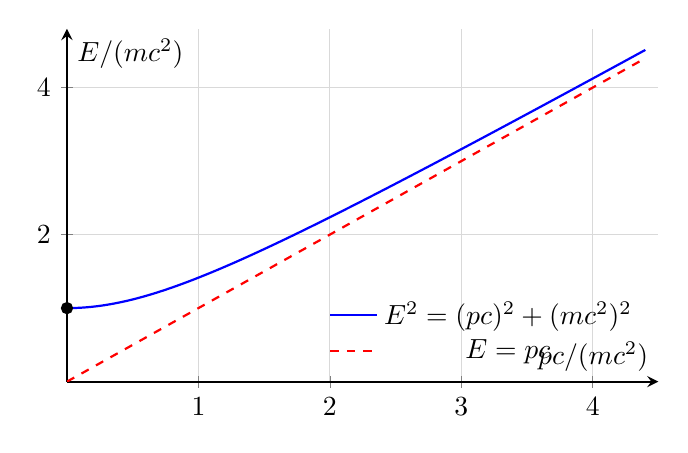
\begin{tikzpicture}
\begin{axis}[
  width=0.75\textwidth, height=0.5\textwidth,
  xlabel={$pc/(mc^2)$}, ylabel={$E/(mc^2)$},
  xmin=0, xmax=4.5, ymin=0, ymax=4.8,
  axis lines=middle,
  grid=major, grid style={gray!30},
  thick,
  legend style={at={(0.98,0.02)}, anchor=south east, draw=none, fill=none}
]
\addplot[blue, domain=0:4.4, samples=200] {sqrt(1 + x^2)};
\addlegendentry{$E^2=(pc)^2+(mc^2)^2$}
\addplot[red, dashed, domain=0:4.4, samples=200] {x};
\addlegendentry{$E=pc$}
\addplot[only marks, mark=*, mark size=1.8pt] coordinates {(0,1)};
\node[anchor=east] at (axis cs:0,1) {$mc^2$};
\end{axis}
\end{tikzpicture}
\caption{固定静质量粒子的能量--动量关系双曲线}
\end{figure}

上图中，蓝色曲线表示固定静质量 $m$ 的粒子在 $(pc,E)$ 平面中的允许状态；红色虚线表示无静质量粒子的情形。它们共同展示了一个事实：在相对论中，能量和动量不是彼此独立的数据，而是由同一个几何结构约束在一起。

\begin{example}[光子的动量]
设一光子的能量为 $E$。由于光子静质量为零，能量--动量关系给出
\[
E=pc.
\]
因此它的动量大小为
\[
p=\frac{E}{c}.
\]
这解释了为什么光照射到物体上能够施加压力：即使没有静质量，光子依然具有动量。
\end{example}

作为一个简短计算，若某粒子的总能量为 $E=3mc^2$，则由
\[
E=\gamma mc^2
\]
立刻得 $\gamma=3$，从而
\[
\frac{1}{\sqrt{1-v^2/c^2}}=3
\quad\Longrightarrow\quad
1-\frac{v^2}{c^2}=\frac19,
\]
故
\[
\frac{v^2}{c^2}=\frac89,
\qquad
v=\frac{2\sqrt{2}}{3}c\approx 0.943c.
\]
这说明总能量达到静能的三倍时，粒子已经处于高度相对论性运动状态。

\section{四矢量}

狭义相对论真正优雅之处，在于它能把许多看似分散的公式统一到四维几何语言之中。时间坐标不再独立于空间坐标，能量也不再独立于动量。描述这种统一最自然的工具就是\emph{四矢量}。

\begin{definition}[四位置]
事件在时空中的四位置定义为
\[
x^\mu=(ct, x, y, z),
\]
也可写作
\[
X=(ct,\vb{x}).
\]
其闵可夫斯基间隔为
\[
X\cdot X = c^2 t^2 - x^2 - y^2 - z^2.
\]
\end{definition}

若粒子沿世界线运动，以其固有时 $\tau$ 为参数，则四速度定义为
\[
U^\mu = \dv{x^\mu}{\tau}.
\]
由于
\[
\dd \tau = \dd t\sqrt{1-v^2/c^2}=\frac{\dd t}{\gamma},
\]
可得
\[
U^\mu = \gamma(c, \vb{v}).
\]

\begin{definition}[四速度与四动量]
粒子的四速度与四动量分别定义为
\[
U^\mu = \gamma(c,\vb{v}),
\qquad
P^\mu = mU^\mu = \left(\frac{E}{c},\vb{p}\right).
\]

其中四动量的时间分量是 $E/c$，空间分量是通常的三维动量 $\vb{p}$。
\end{definition}

四动量的“长度”是不变的：
\[
P^\mu P_\mu = \left(\frac{E}{c}\right)^2-p^2 = m^2c^2,
\]
这正是上一节能量--动量关系的四维写法。

\begin{law}[四动量守恒]
在任意孤立体系中，总四动量守恒：
\[
\sum_i P_i^\mu\bigg|_{\text{初}}=
\sum_j P_j^\mu\bigg|_{\text{末}}.
\]
它同时包含了能量守恒与三维动量守恒，而且比二者分别书写更具有坐标无关性。
\end{law}

这条定律是粒子物理分析的核心。因为四动量守恒一旦在一个惯性系中成立，它就在所有惯性系中自动成立。

\begin{remark}
牛顿力学中的动量守恒与能量守恒，看上去是两条不同定律；在相对论中，它们是同一个四维守恒定律的不同分量。统一，正是现代物理最深刻的特征之一。
\end{remark}

\begin{example}[四速度与四动量的计算]
质量为 $m$ 的粒子以 $0.60c$ 沿 $x$ 方向运动。求其四速度和四动量。

由
\[
\gamma=\frac{1}{\sqrt{1-0.60^2}}=1.25,
\]
得
\[
U^\mu = \gamma(c,v,0,0)=\bigl(1.25c,0.75c,0,0\bigr).
\]
故四动量为
\[
P^\mu = mU^\mu = \bigl(1.25mc,0.75mc,0,0\bigr).
\]
于是总能量与三动量分别为
\[
E=1.25mc^2,
\qquad
p_x=0.75mc.
\]
\end{example}

\section{相对论碰撞与衰变}

在经典力学中，碰撞问题依靠能量守恒和动量守恒；在相对论中，最有效的方法是直接使用四动量守恒。这样既避免了繁琐的速度变换，也能自动照顾到静能与质量变化。

设某反应写作
\[
a+b\to 1+2+\cdots+n.
\]
则四动量守恒为
\[
P_a^\mu+P_b^\mu = \sum_{k=1}^{n} P_k^\mu.
\]
把两边平方，便可构造参考系无关的不变量，这在阈值能、衰变产物能谱、反应可否发生等问题中尤其有力。

\subsection*{一、两体衰变}

考虑一个静止粒子 $A$ 衰变为两个粒子：
\[
A\to 1+2.
\]
在 $A$ 的静止系中，初态四动量为
\[
P_A^\mu=(M c,\vb{0}),
\]
其中 $M$ 是母粒子质量。守恒律给出
\[
\vb{p}_1+\vb{p}_2=\vb{0},
\]
因此两个子粒子的动量大小相等、方向相反。这说明衰变并不是“随便飞开”，而是受到严格几何约束。

\begin{center}
\begin{tikzpicture}[scale=1.0, >=Stealth]
  \draw[->, thick] (-2,0) -- (0,0) node[midway, above] {$A$};
  \fill (0,0) circle (1.6pt);
  \draw[->, thick, blue] (0,0) -- (2,1.2) node[midway, above] {$1$};
  \draw[->, thick, red] (0,0) -- (2,-1.2) node[midway, below] {$2$};
  \node at (0.25,0.35) {$\star$};
  \node[blue!70!black] at (1.4,1.55) {$\vb{p}_1$};
  \node[red!70!black] at (1.4,-1.55) {$\vb{p}_2$};
\end{tikzpicture}
\end{center}

进一步可得子粒子的能量：
\[
E_1 = \frac{M^2+m_1^2-m_2^2}{2M}c^2,
\qquad
E_2 = \frac{M^2+m_2^2-m_1^2}{2M}c^2.
\]
若 $m_1=m_2$，则两者平分总能量。

\subsection*{二、湮灭与产生}

电子与正电子静止湮灭时，初态总动量为零。若末态只有一个光子，则该光子动量不可能为零，因此违背动量守恒。于是最简单允许过程必须是
\[
e^-+e^+\to \gamma+\gamma,
\]
并且两个光子沿相反方向飞出，各自携带相等的能量。这个结论完全来自四动量守恒。

反过来，高能光子或粒子束也可以在碰撞中产生新粒子，只要初态总能量足够，且四动量守恒可满足。现代粒子加速器正是利用这一点，把动能“浓缩”进碰撞区，转化为新的粒子质量与运动能量。

\begin{example}[静止电子--正电子对的湮灭]
设电子和正电子都处于静止状态。各自静能为 $mc^2$，初态总四动量为
\[
P_{\text{ini}}^\mu = (2mc,\vb{0}).
\]
末态若为两个反向光子，则设每个光子能量为 $E_\gamma$，动量大小为 $E_\gamma/c$。由动量守恒知二者方向相反，由能量守恒知
\[
2E_\gamma = 2mc^2.
\]
因此
\[
E_\gamma = mc^2.
\]
这说明静质量可以完整地转化为辐射能，但总四动量依然守恒。
\end{example}

\begin{example}[母粒子静止系中的双光子衰变]
若某中性粒子静止时衰变为两个光子，
\[
A\to \gamma+\gamma,
\]
设其质量为 $M$。由于初态总动量为零，末态两个光子必须反向发射，且两者能量相等。由能量守恒得
\[
2E_\gamma = Mc^2,
\qquad
E_\gamma = \frac12 Mc^2.
\]
于是每个光子的动量大小为
\[
p_\gamma = \frac{E_\gamma}{c}=\frac12 Mc.
\]
这类过程在粒子物理与核物理中都极其常见。
\end{example}

\begin{remark}
四动量方法最大的优势，在于它不依赖某个特别“好算”的参考系。实际计算时，我们常先在质心系中利用对称性求解，再把结果变换到实验室系。这个流程，是现代高能物理最基本的工作语言。
\end{remark}

\section{从牛顿到爱因斯坦：回顾与展望}

现在回头看全书，我们已经走完了一条非常清晰的思想路线。

在前几章中，我们从微积分的语言重新整理了经典力学：位置、速度、加速度是导数，位移与功是积分；牛顿定律给出运动方程，动量守恒与能量守恒提供整体视角。接着我们进入电磁学，看到电场、磁场、感应与麦克斯韦方程如何把分散现象统一为一个连续场论。最后，正是麦克斯韦理论中光速不变的结构，迫使我们重新审视时间与空间本身。

于是，爱因斯坦迈出了决定性的一步：
\begin{itemize}
  \item 时间不再绝对；
  \item 空间不再绝对；
  \item 质量、能量、动量被统一进时空几何；
  \item 守恒律被提升为四维协变的形式。
\end{itemize}

这并不意味着牛顿错了，而是意味着牛顿理论有自己的适用范围。正如欧几里得几何在平坦空间中极其有效，牛顿力学在低速、弱场、宏观尺度下仍然是最强大、最实用的近似理论之一。爱因斯坦做的，是告诉我们当速度接近光速、当精度要求更高时，自然界采用的是一个更深的结构。

\begin{theorem}[经典极限原则]
当 $v/c\to 0$ 且作用尺度远离相对论与量子效应时，狭义相对论的动力学方程退化为牛顿力学：
\[
\vb{p}=\gamma m\vb{v}\to m\vb{v},
\qquad
E=\gamma mc^2 \to mc^2 + \frac12 mv^2.
\]
因此，新理论不是否定旧理论，而是包含并修正旧理论。
\end{theorem}

但故事并没有结束。狭义相对论只处理\emph{惯性系}中的物理规律，且假定时空本身是平直的。接下来，若我们继续追问两个更深的问题，就会走向二十世纪物理学的另外两座高峰：
\begin{enumerate}
  \item 如果引力不是一种普通力，而是时空几何的弯曲，会发生什么？
  \item 如果微观世界不遵循确定轨道，而遵循概率振幅，又会发生什么？
\end{enumerate}

第一个问题通向\emph{广义相对论}。在那里，引力不再被理解为远距离作用的神秘拉力，而是质量与能量告诉时空如何弯曲，弯曲的时空再告诉物体如何运动。行星轨道、引力红移、黑洞、引力波，都是这一思想的果实。

第二个问题通向\emph{量子力学}。在那里，粒子既像粒子又像波，测量不再只是“读取结果”，而会参与物理量的呈现；原子结构、化学键、半导体、激光，乃至现代信息技术，都建立在这种新的微观规律之上。

而当狭义相对论与量子力学进一步结合，我们又会抵达\emph{量子场论}：粒子成为场的激发，反应过程成为对称性与守恒律的精确表达。你在本章学到的四动量守恒，正是那门理论中最基本、最稳定、最经久不衰的骨架之一。

\begin{remark}
物理学最迷人的地方，不在于公式越来越复杂，而在于世界图景越来越统一。从牛顿的力，到麦克斯韦的场，再到爱因斯坦的时空，我们一步步看到：自然界并不零碎，它在更深处总会显出简洁的秩序。
\end{remark}

如果这本书完成了它的使命，那么你现在应该不仅会计算，更会追问：为什么要这样定义？为什么守恒律如此重要？为什么新的理论必须在旧理论成功的地方保持成功？这些问题，正是进入真正理论物理学习的门槛。

愿你带着这种追问继续前行。前方等待你的，也许是黎曼几何中的引力，也许是希尔伯特空间中的量子态，也许是粒子对撞机里一闪而过的新粒子。但无论走到哪里，你都已经掌握了一条最重要的线索：\emph{用数学结构去读懂自然规律}。

